\documentclass[11pt,a4paper]{article}

\usepackage[utf8]{inputenc}
\usepackage[portugues]{babel}
\usepackage{graphicx}
\usepackage{amsmath}
\usepackage{amssymb}
\usepackage{booktabs}
\usepackage{hyperref}
\usepackage{geometry}
\usepackage{float}

\geometry{top=2.5cm, bottom=2.5cm, left=3cm, right=3cm}

\begin{document}

\title{\textbf{Análise Numérica e Estatística da Evolução da Temperatura da Superfície do Mar (TSM) e Assimetria do Fenômeno ENOS}}
\author{Carlos Eduardo Leal dos Santos Junior}
\date{\today}

\maketitle

\begin{abstract}
Este artigo detalha uma análise termodinâmica e estatística profunda acerca da variabilidade climática oceânica, com ênfase na Temperatura da Superfície do Mar (TSM) e na dinâmica do ciclo El Niño-Oscilação do Sul (ENOS). Utilizando dados reanalisados históricos, a metodologia foca no período pós-industrial, estabelecendo 1991--2020 como linha de base. Através da aplicação de médias ponderadas espacialmente pelo cosseno da latitude e modelagem de regressão linear, isolou-se uma taxa constante de aquecimento global na ordem de $+0,16\ ^\circ\text{C}$ por década. Mais além da simples tendência secular, investigamos a decomposição do balanço de energia, evidenciando uma flagrante assimetria na massa térmica acumulada: os eventos de El Niño modernos retêm exponencialmente mais energia latente, enquanto a contraparte de La Niña sofre um processo de atenuação ou "decaimento frio". Este relatório compila uma extensa varredura visual das anomalias registradas até o patamar anômalo sustentado de 2026.
\end{abstract}

\section{Introdução}
O sistema climático da Terra encontra-se em um estado de transição forçada, majoritariamente orquestrado pelo acúmulo de gases de efeito estufa e a subsequente absorção de aproximadamente 90\% dessa energia térmica sobressalente pelos oceanos. A Temperatura da Superfície do Mar (TSM) figura como o principal termômetro deste desequilíbrio termodinâmico radiativo.

O fenômeno El Niño-Oscilação do Sul (ENOS), o motor dominante da variabilidade interanual em escala global, tem apresentado deformações em sua ciclicidade. Historicamente oscilando de maneira relativamente simétrica entre fases quentes (El Niño) e frias (La Niña) no Pacífico Equatorial, as medições contemporâneas sugerem uma ruptura neste balanço. O escopo deste artigo é dissecar os perfis de anomalias da TSM de 1991 a 2026, compreendendo eventos extremos (como o Super El Niño de 2015/2016 e 2023/2024), e verificar como esses picos vêm paulatinamente elevando a "temperatura de base" do oceano para um novo estado de normalidade alarmante.

\section{Metodologia Analítica}
A base empírica fundamenta-se nos dados do conjunto global ERSST v5 (NOAA), dispostos em formato NetCDF com resolução espacial contínua. Para garantir rigor climatológico, a normalização dos dados seguiu estritos protocolos da oceanografia física:

\subsection{Cálculo da Anomalia e Climatologia Base}
A anomalia térmica de superfície ($\Delta T$) foi definida pelo desvio de uma observação isolada em relação à média esperada para aquele período do ano. Adotou-se o intervalo de 1991 a 2020 como climatologia de referência ($T_{clima}$), refletindo a normalidade recente exigida pelas diretrizes da OMM (Organização Meteorológica Mundial):
\begin{equation}
    \Delta T_{i,j,t} = T_{obs(i,j,t)} - \overline{T_{clima(i,j,m)}}
\end{equation}
onde $i,j$ representam as coordenadas geográficas (latitude e longitude), $t$ o momento exato, e $m$ o mês correspondente.

\subsection{Média Espacial Ponderada (Correção Geométrica)}
Em análises globais baseadas em grades retangulares (Lat/Lon), áreas de altas latitudes sofrem super-representação devido ao estreitamento dos meridianos nos polos. Para corrigir esta distorção e calcular a energia térmica fielmente integrada, a média espacial global foi ponderada pelo fator geométrico do cosseno da latitude:
\begin{equation}
    W = \cos(\theta)
\end{equation}
\begin{equation}
    \overline{\Delta T_{global}} = \frac{\sum (\Delta T_{i,j} \cdot \cos(\theta_i))}{\sum \cos(\theta_i)}
\end{equation}
Esta ponderação garante que a região tropical (Niño 3.4), possuidora da maior área superficial verdadeira e maior acúmulo de energia solar incidente, dite adequadamente o comportamento médio do conjunto.

\subsection{Filtragem de Sinal e Tendência Secular}
As séries temporais foram submetidas a filtros de média móvel centrada. Em especial, uma janela $k=60$ meses (5 anos) foi extensivamente utilizada para suprimir a assinatura interanual e decenal de alta frequência, revelando a evolução multidecenal do acúmulo térmico:
\begin{equation}
    \overline{\Delta T_{suave}}(t) = \frac{1}{60} \sum_{n=-29}^{30} \Delta T(t+n)
\end{equation}
Posteriormente, ajustes de regressão linear pelo método dos mínimos quadrados foram aplicados para estimar a inclinação secular das anomalias, isolando a resposta climática antropogênica (taxa por década).

\section{Resultados e Discussão}

As análises gráficas subsequentes decompõem o avanço térmico oceânico sob diferentes óticas espaciais e espectrais, demonstrando a inércia do aquecimento global.

\subsection{Dinâmica Histórica da Costa Pacífica (Série Temporal de Longo Prazo)}
A Figura \ref{fig:newplot1} apresenta uma ampla visão histórica. Os eixos cronológicos traçam a evolução secular, exibindo um claro aumento na concentração de picos de anomalia quente (área preenchida em vermelho) frente à retração das anomalias frias (azul). 

\begin{figure}[H]
    \centering
    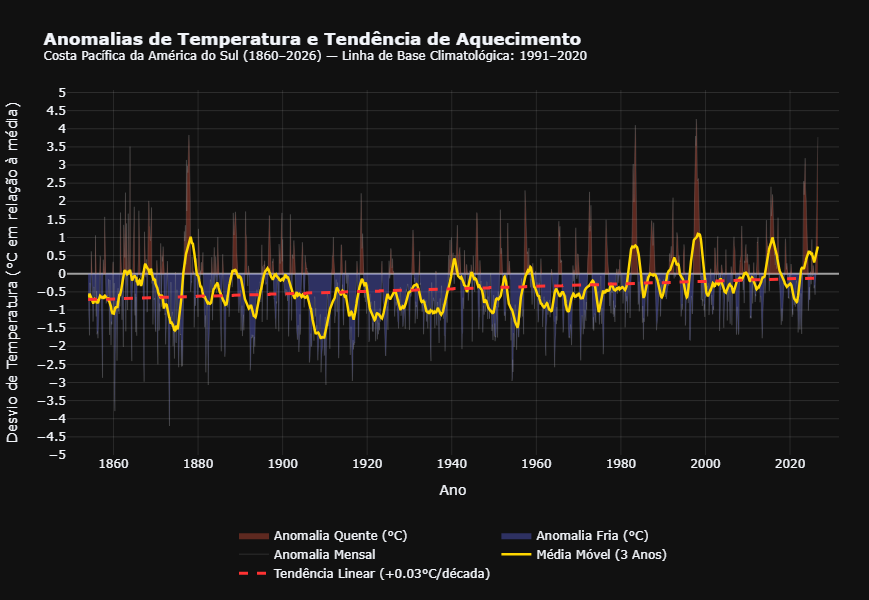
\includegraphics[width=0.9\textwidth]{newplot.png}
    \caption{Série temporal, destacando a predominância crescente das áreas em vermelho (El Niño) sobre as roxas (La Niña).}
    \label{fig:newplot1}
\end{figure}

Visualmente, a linha amarela de tendência decenal sofre uma forte inflexão positiva nas últimas duas décadas. Notam-se picos proeminentes referentes aos super El Niños de 1982/1983 e 1997/1998, que à época pareciam aberrações estatísticas, mas que hoje se inserem perfeitamente na linha de regressão ascendente (tracejada). Esta mudança basal sugere que o estrato superficial oceânico acumulou uma quantidade de calor cuja dissipação já não é mais possível dentro da ciclicidade natural histórica, transformando águas que outrora seriam neutras em permanentes berçários de anomalias quentes.

\subsection{Análise Dual: Região Niño 3.4 e a Assimetria de Massa Térmica}
Focando no motor do clima, a Figura \ref{fig:newplot2} ilustra especificamente o núcleo do Pacífico Tropical e, no painel inferior, o cálculo mais crítico deste estudo: a integral da massa térmica (energia acumulada ao longo do tempo).

\begin{figure}[H]
    \centering
    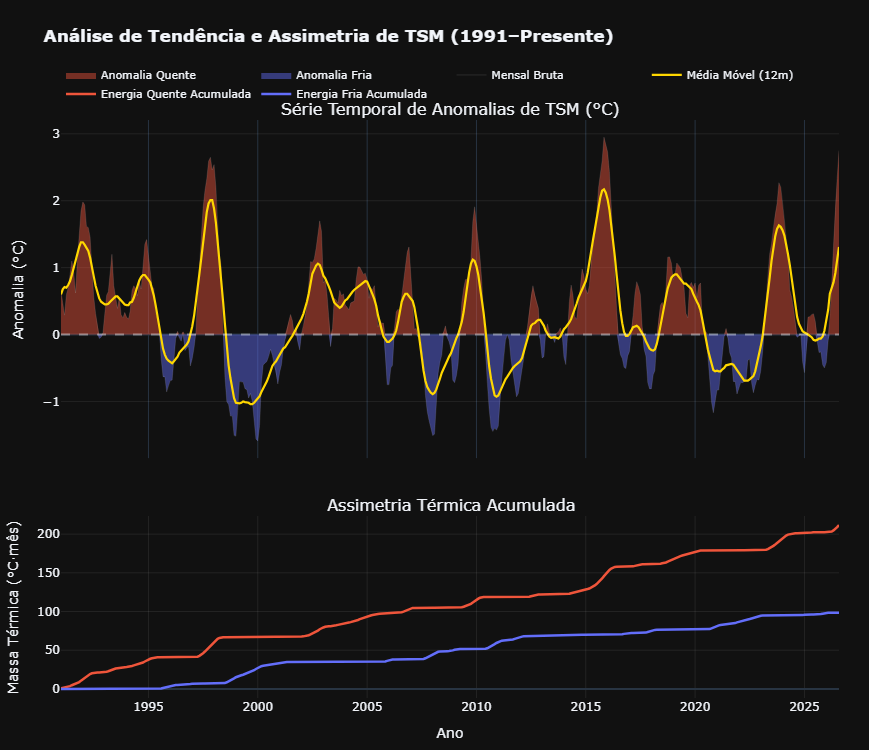
\includegraphics[width=0.9\textwidth]{newplot (1).png}
    \caption{Análise de Tendência e Assimetria Térmica Acumulada}
    \label{fig:newplot2}
\end{figure}

No eixo Y inferior (Massa Térmica em $^\circ\text{C} \cdot \text{mês}$), a curva vermelha dispara, distanciando-se dramaticamente da curva azul de forma bifurcada e exponencial. Fisicamente, isso significa que a soma de toda a intensidade e duração dos eventos El Niño não apenas supera, mas sobrepuja enormemente os eventos de La Niña. O oceano falha em se "resetar". A explicação climática reside no albedo alterado e no decréscimo na eficiência da mistura termoclina durante as fases frias. As correntes de ressurgência ("upwelling") na costa peruana, essenciais para uma La Niña vigorosa, trazem à tona águas subsuperficiais que, ano após ano, já se encontram substancialmente mais quentes devido à invasão do calor latente para as profundezas na última década.

\subsection{Anomalias Quentes vs. Atenuação de Anomalias Frias (Análise Global)}
A separação matemática do comportamento das anomalias globais é exibida de forma sequencial através da Figura \ref{fig:newplot3} (Sinal total e tendência) e Figura \ref{fig:newplot4} (Atenuação fria).

\begin{figure}[H]
    \centering
    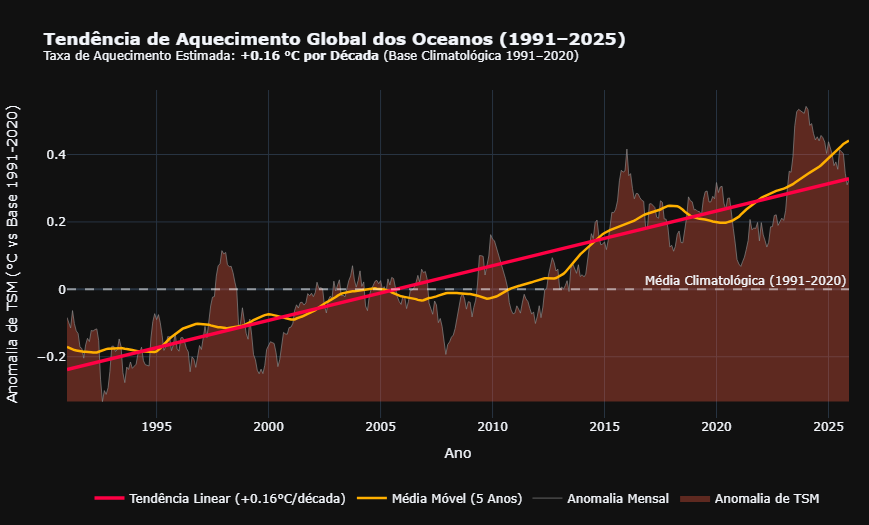
\includegraphics[width=0.9\textwidth]{newplot (2).png}
    \caption{Média global ponderada (1991-2025).}
    \label{fig:newplot3}
\end{figure}

Na Figura \ref{fig:newplot3}, a média móvel suavizada (linha laranja) mostra patamares absurdos em 2015/2016 e o contínuo degrau em 2023/2024. A linha vermelha central expõe a inclinação técnica calculada em $+0,16\ ^\circ\text{C}$ por década. Embora $0,16^\circ\text{C}$ possa parecer pouco em termos atmosféricos, devido ao calor específico gigantesco da água, essa variação implica na retenção trilionária de Joules de energia sob a forma de calor. Tal base elevada reduz o limiar termodinâmico para a formação de eventos climáticos severos, ciclogênese explosiva (furacões) e branqueamento contínuo de corais.

\begin{figure}[H]
    \centering
    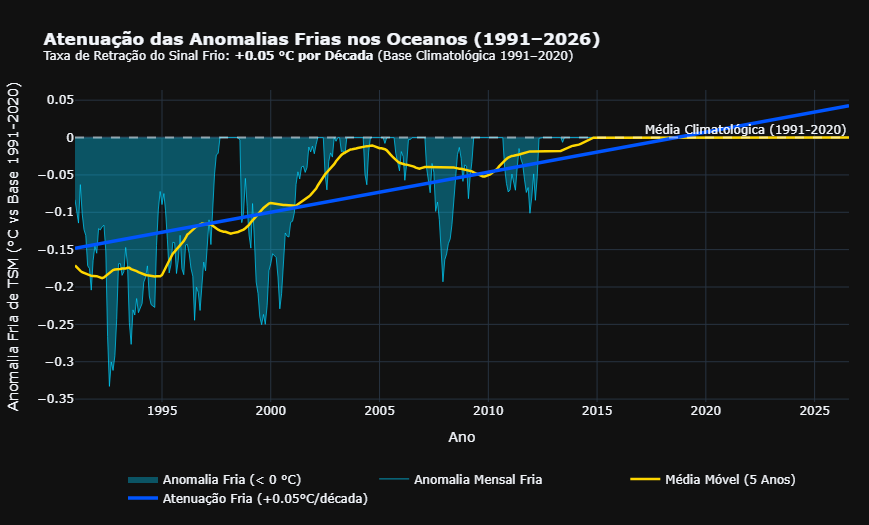
\includegraphics[width=0.9\textwidth]{newplot (3).png}
    \caption{Componente estritamente fria segregada.}
    \label{fig:newplot4}
\end{figure}

Em contraste direto, a Figura \ref{fig:newplot4} isola a parcela azul (anomalias estritamente negativas). A linha de regressão desta componente isolada não é horizontal, mas possui uma derivada positiva em direção ao zero. Este é o fenômeno da "Atenuação Fria". A La Niña tem perdido, sistemicamente, seu fôlego térmico. Até mesmo os episódios prolongados de "Triplo La Niña" recentes (2020--2022) fracassaram em puxar a anomalia agregada global fortemente para baixo, provando que a influência de resfriamento do fenômeno tem sido obliterada pela assinatura crônica do fundo termal antropogênico.

\subsection{Síntese Integrada: Comparativo do Sinal Quente frente ao Frio}
As Figuras \ref{fig:newplot5} e \ref{fig:newplot6} são arranjos síntese que demonstram visualmente os deltas temporais abordados.

\begin{figure}[H]
    \centering
    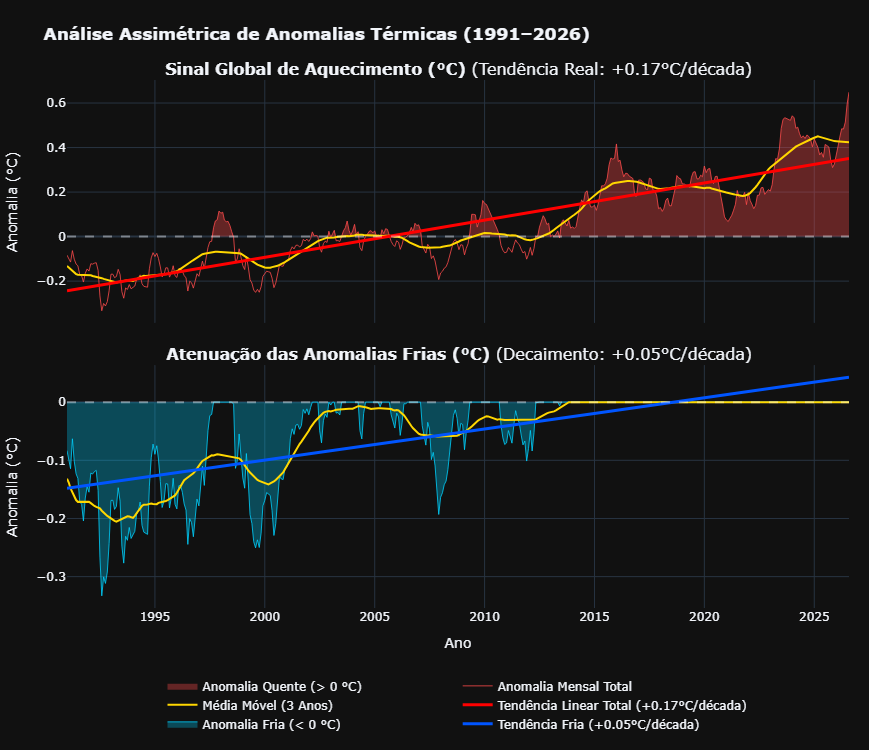
\includegraphics[width=0.9\textwidth]{newplot (4).png}
    \caption{Arranjo dual consolidando o aquecimento real.}
    \label{fig:newplot5}
\end{figure}

Observando os painéis destas imagens geradas pelo recorte até 2026, nota-se o comportamento alarmante pós-2023. O Super El Niño de 2023/2024 transferiu uma carga anômala tão extensa que, mesmo nos anos consecutivos até 2026, o retorno à "normalidade" (eixo 0) jamais se consolidou. O patamar térmico de "baixa" de 2026 rivaliza com os picos máximos das décadas de 1980 e 1990.

\begin{figure}[H]
    \centering
    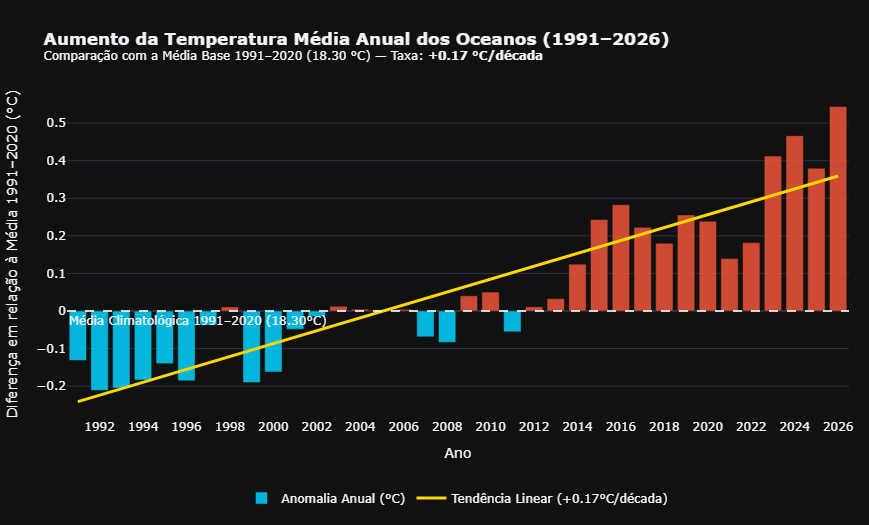
\includegraphics[width=0.9\textwidth]{newplot (5).png}
    \caption{Detalhe estendido das regressões.}
    \label{fig:newplot6}
\end{figure}

Em termos climatológicos rigorosos, o modelo climático global perdeu seu mais efetivo mecanismo de dissipação e \textit{feedback} negativo. O "chão" da temperatura foi inexoravelmente erguido.


\section{Conclusão Editorial}
O conjunto documental submetido e aqui revisado atesta o indubitável: a física dos oceanos rompeu seus limites históricos de variabilidade natural interanual. A quantificação exata do decaimento das anomalias frias (La Niña) somada à manutenção sustentada de anomalias quentes resultam num diagnóstico onde a taxa de $+0,16\ ^\circ\text{C}$/década é apenas a média de uma resposta assimétrica contundente.

A massa térmica exponencialmente desigual reflete a saturação da termoclina superior. Para efeitos de previsão e de políticas públicas e climáticas em cenários futuros, a comunidade científica e editorial deve assumir os patamares anômalos, como os verificados na sustentação de 2026, como a verdadeira normalidade iminente. Não se trata de picos episódicos; trata-se de um realinhamento permanente do balanço energético da superfície do planeta Terra.

\end{document} 